%\documentclass[reponses, utf8, 11pt]{feuille}
\documentclass[utf8, 11pt]{feuille}

\newcommand{\titredutd}{\textbf{TD10 --- Le modèle d'Ising}}

\begin{document}


\begin{tcolorbox}[
        colback=gray!20,
        colframe=gray!20,
        width=\dimexpr\textwidth\relax, 
        arc=0pt,outer arc=0pt,
        ]

\texttt{Seules les calculatrices non communicantes et les notes manuscrites personnelles sont autorisées.}

\texttt{Les exercices sont totalement indépendants.}

\texttt{On notera $k_B$ la constante de Boltzmann et $h$ la constante de Planck.}

\end{tcolorbox}



% ______________________________________________________________________________
\section{\medium~Le modèle d'Ising en champ moyen}

Le modèle d'Ising est le cadre le plus simple pour étudier la transition de phase ferromagnétique-paramagnétique. Le système est formé de $N \gg 1$ atomes localisés aux n\oe uds d'un réseau cristallin de coordinence $q$ (le nombre de plus proches voisins). Chaque atome $i$ porte un moment magnétique $\mu_i$ ne pouvant prendre que deux valeurs $\mu_i= \pm \mu$ (spin $\frac{1}{2}$). Le système est plongé dans un champ magnétique extérieur $B$ et est en contact avec un thermostat à la température $T$. L'hamiltonien du modèle d'Ising, suggéré par Wilhelm Lenz vers 1924 à son étudiant en thèse Ernst Ising, s'écrit
$$
H=-J\sum_{\langle i,j \rangle}\mu_i \mu_j -B\ \sum_{i=1}^N \mu_i \quad \textrm{avec} \quad J>0
$$
où ${\langle i,j\rangle}$ indique que la somme est prise sur toutes les paires de sites plus proches voisins.

\medskip

\question
Dans quel micro-état l'énergie du système est-elle minimale ? Que vaut alors dans cette configuration le moment magnétique moyen $m=\langle \mu_i \rangle$ ?

\question
Exprimer la fonction de partition $Z$ du système à l'équilibre avec un thermostat à la température $T$. On note $\beta=\frac{1}{k_B T}$. Pourquoi ne peut-on pas la calculer en général ?

\question
Dans le cas de l'hamiltonien ci-dessus, l'approximation de champ moyen s'obtient à partir de l'identité
$$
\mu_i\mu_j = (\mu_i -m)(\mu_j -m)+ m(\mu_i+\mu_j)-m^2
$$
où $m=\langle \mu_i \rangle$ est la valeur moyenne du moment magnétique, que l'on cherche à déterminer dans la suite.  Montrer qu'en négligeant le terme $(\mu_i -m)(\mu_j -m)$, l'hamiltonien se réécrit 
$$
H \simeq \sum_{i=1}^N h_i \quad \textrm{avec} \quad h_i= -(Jqm+B) \mu_i
+J\frac{q}{2} m^2
$$

\question
Calculer alors la fonction de partition $Z_{\rm cm}$ et l'énergie libre $F_{\rm cm}$.

\question
Exprimer le moment magnétique moyen $m$ comme une dérivée partielle de $F$ et en déduire l'équation auto-cohérente :
\begin{equation} \label{eqAutoIsing}
m=\mu \tanh  \big[ \beta \mu(J q m +B) \big]
\end{equation}

\question
Pour résoudre graphiquement l'équation auto-cohérente (\ref{eqAutoIsing}) en {\it champ nul} (pour $B=0$), introduire la variable $x=\beta  J q \mu m$  et tracer $y_1(x)=\frac{x}{\beta  J q \mu^2}$ et $y_2(x)=\tanh (x) $. Montrer que résoudre (\ref{eqAutoIsing}) revient à chercher l'intersection des courbes $y_1(x$) et $y_2(x)$. Montrer que pour $T> T_c =\frac{Jq\mu^2}{k_B}$ il n'y a qu'une solution $m=0$ et que pour $T< T_c$ il y a trois solutions, $m=0$ et $m=\pm m_s(T)$, que l'on ne cherchera pas à calculer.  Pourquoi parle-t-on de brisure de symétrie ?

\question
Tracer $F_{\rm cm}(m)$, dont l'expression a été obtenue à la question précédente, et montrer que les seules solutions stables pour $T<T_c$ sont $m=\pm m_s(T)$.  La courbe de $\frac{m(T)}{\mu}$ est représentée sur la figure ci-dessous. Commenter l'accord avec les données expérimentales présentées.

\begin{figure}[h!]
\centering
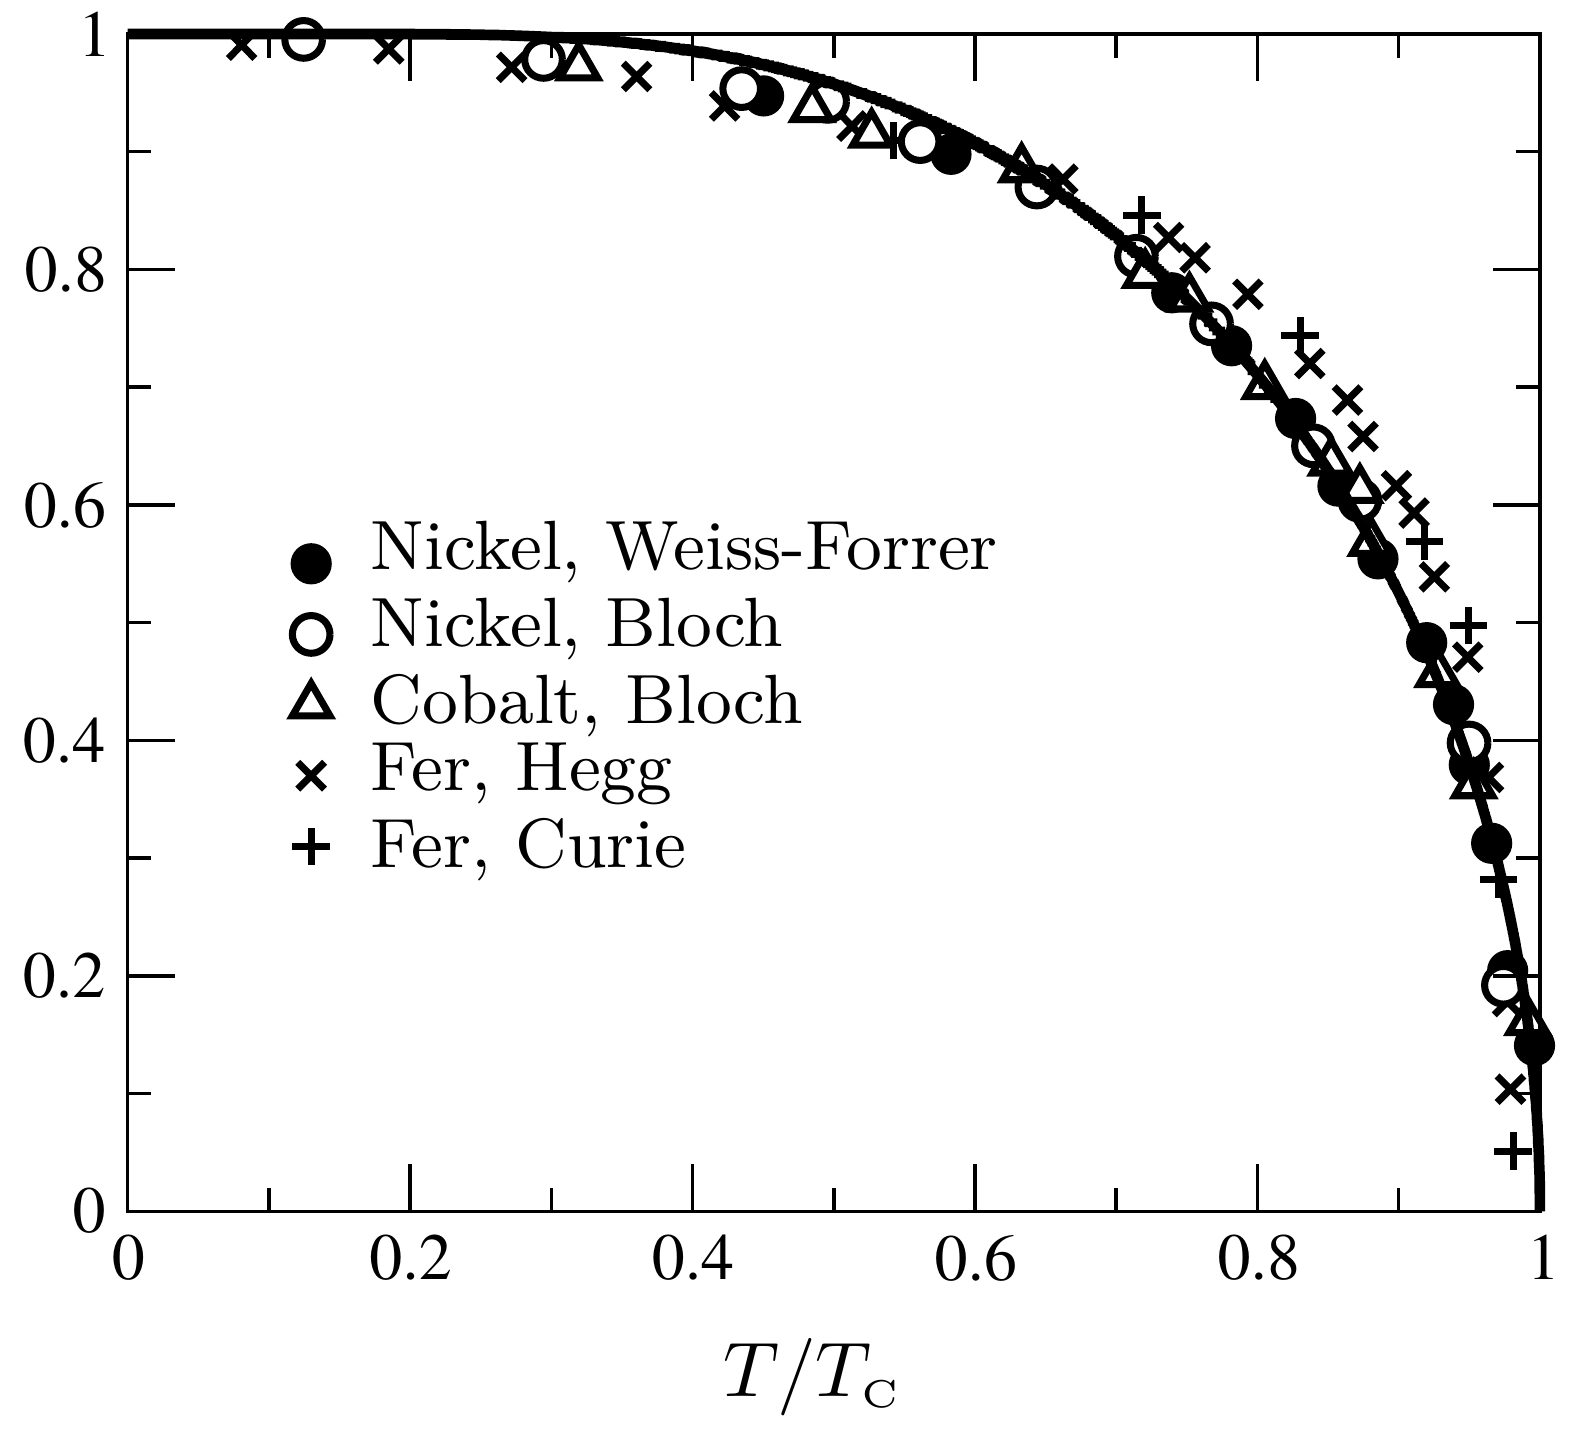
\includegraphics[scale=0.6,angle=0]{ising}
\caption{Aimantation spontanée $\frac{m(T)}{\mu}$ de plusieurs substances ferromagnétiques en fonction de la température $\frac{T}{T_c}$, où $T_c=1043$ K pour le fer, $T_c=650$ K pour le nickel, $T_c=1415$ K pour le cobalt. Le trait plein correspond à la solution numérique, $m_s(T)$, de l'équation (\ref{eqAutoIsing}). Les points sont les résultats expérimentaux obtenus par les auteurs mentionnés dans la légende (d'après Sator$\&$Pavloff (Vuibert, 2016)).}
\end{figure}

\question
\'Ecrire un développement limité de l'équation auto-cohérente (\ref{eqAutoIsing}) au voisinage du point critique (où $m \simeq 0$) et montrer que $m\sim (T_c-T)^{\beta}$ pour $T<T_c$, où $\beta$ (et oui... terrible comme notation n'est-ce pas ?) est un exposant critique dont on déterminera la valeur. Dépend-elle du matériau considéré ?  

\question
Calculer la dérivée partielle $\displaystyle \frac{\partial m}{\partial B}\Big|_{T}$ en fonction de $m$, $T$ et $B$ à l'aide de l'équation (\ref{eqAutoIsing}) et en déduire la susceptibilité magnétique en champ nul (pour $B=0$), $\displaystyle \chi=\frac{\partial m}{\partial B}\Big|_{T}$, en fonction de $T$. Montrer qu'au voisinage du point critique $\chi \sim |T-T_c|^{-\gamma}$, où $\gamma$ est un exposant critique dont on déterminera la valeur (on distinguera les cas $T>T_c$ et $T<T_c$). 

\question
Amorcer l'étude en champ magnétique non nul (pour $B \ne 0$). Montrer notamment qu'il existe toujours une unique solution d'aimantation non nulle dans le sens du champ, quelle que soit la température, et justifier que la variation de cette aimantation ne présente pas de singularité en fonction de la température. 


\end{document}
